% Deve resumir o experimento, os resultados e a discussão (comentários)
% e incluir opiniões do grupo e propostas futuras para o experimento
%Descrição do hardware
%Descrição do software
%\cite{Advpdf}
%\cite{thepdf}
%\cite{dsl}

\subsection{Estruturas}\label{struct}

\subsubsection{Arquitetura}\label{arq}

No intuito de manter o jogo compatível com qualquer sistema operacional, foi decidido centralizar as inclusões de bibliotecas em um único arquivo. Para essa função foi criado o arquivo \textit{"defines.h"}, que é responsável por reconhecer o sistema em que esta sendo compilado e incluir os devidos \textit{headers}.

\begin{lstlisting}[language=C++,title=\textit{defines.h},firstnumber=5,numbers=none]
#if defined (__APPLE__) || defined (MACOSX) /*MAC OS*/
    #include <GLUT/glut.h>
#else
    #ifdef _WIN32                           /* Windows */
    	#define WIN32_LEAN_AND_MEAN
        #include <glee.h>
        #include <gl/gl.h>
		#include <gl/glut.h>
        #include <windows.h>
        #define sleep(x) Sleep(x)
    #else                                   /*Linux*/
    	#include <cstdarg>
    	#include <unistd.h>
        #include <GL/gl.h>
        #include <GL/glut.h>
        #include <GL/glu.h>
        #define Sleep(x) usleep(x<1000000?10000+300*x:x)
    #endif
#endif
\end{lstlisting}

No trecho mostrado acima, podemos ver como o programa reconhece em qual sistema esta sendo compilado e em qual endereço irá procurar pelas bibliotecas. A decisão é tomada de forma bem simples e objetiva, buscando apenas saber se as definições \textbf{MACOSX} ou \textbf{\_WIN32} existem. Com estas duas definições é suficiente para dividir entre os três sistemas operacionais que o programa se propõe a dar suporte. 

Porém este não é o único problema enfrentado quando se trata de um programa multiplataforma, mas também existem as dificuldades com a própria compilação.

Visando isso, foi feito um arquivo \textit{makefile} que procede com teste semelhante ao feito no \textit{defines.h} para verificar em que sistema se encontra e assim efetuar os links corretamente. Um trecho do \textit{makefile} pode ser observado a seguir:

\begin{lstlisting}[language=make,title=\textit{Makefile},firstnumber=8,numbers=none]
UNAME = $(shell uname)
ifeq ($(UNAME),Linux) # Linux OS
	GLFLAGS = -lglut -lglui -lGLU -lGL -lalut -lopenal
	else
	ifeq ($(UNAME),Darwin) # MAC OS X
		GLFLAGS = -framework OpenGL -framework GLUT
	else #Windows
		GLFLAGS = -lopengl32 -lglu32 -lglut32 -lglee -lalut
	endif
endif
\end{lstlisting}

É valido aproveitar a oportunidade para frisar no trecho mostrado acima do \textit{makefile} a inclusão das flags \textit{-lalut -lopenal} para inclusão de áudio no programa.

\subsubsection{Execução}\label{exe}

\paragraph{\textbf{Windows}}

O programa foi desenvolvido com auxilio da IDE \textit{CodeBlocks}\footnote{Acesse \url{http://www.codeblocks.org/} para maiores informações sobre a IDE.}. Assim, para gerar o executável na plataforma, basta abrir o arquivo \textit{Projeto - Labirinto.cbp} no \textit{CodeBlocks} e mandar compilar/construir o projeto. Na própria IDE haverá meios de executar o arquivo de saída, porém na pasta do projeto será possível localizar também o arquivo \textit{*.exe}.

\paragraph{\textbf{Linux}}

Para se construir o programa na plataforma Linux, é necessário ter algumas bibliotecas instaladas no sistema. Dentre elas é valido destacar as do OpenGL e de áudio (\textit{Alut} e \textit{Openal}). Na pasta onde se encontra os arquivos fontes, é possível localizar o arquivo \textit{makefile}. No terminal, basta executar o comando \textbf{make run} no diretorio contendo o arquivo \textit{makefile} para compilar os arquivos e inicializar o programa corretamente. Caso alguma das bibliotecas necessárias não estejam instaladas, será observado a lista de \textit{warnings/errors}, orientando qual biblioteca deve de ser instalada. É valido lembrar que para instalar as bibliotecas para este fim na plataforma Linux, deve-se buscar pelos nomes com o sufixo \textit{-dev}, garantindo assim que serão instalados os arquivos necessários. A compilação será feita de forma silenciosa e se não tiver problemas, apresentará uma saída semelhante a:

\begin{lstlisting}[language=bash,title=\textit{Saída do terminal - Linux},numbers=none]
$ make run
System: Linux OS
compiling...ok
Running...
\end{lstlisting}

\paragraph{\textbf{Mac OS}}

Semelhante aos passos no sistema Linux, o usuário terá que executar o comando \textbf{make run} no diretorio contendo o arquivo \textit{makefile} para compilar os arquivos e inicializar o programa corretamente. Se a compilação ocorrer corretamente, a saída deverá ser semelhante a:

\begin{lstlisting}[language=bash,title=\textit{Saída do terminal - Mac OS},numbers=none]
$ make run
System: Darwin
compiling...ok
Running...
\end{lstlisting}


\subsubsection{Artefatos}\label{artefatos}

\paragraph{\textbf{Arquivos}}

Arquivos utilizados na construção do programa\footnote{Atualizado em 7 de Junho de 2012}:\\

\begin{itemize}
	\item button.cpp
	\item camera.h
	\item entidade.cpp
	\item eventos.h 
	\item gamemanager.cpp  
	\item map.h        
	\item minimap.h   
	\item soundAL.cpp  
	\item text.h             
	\item tile.cpp   
	\item vetor.h
	\item button.h    
	\item defines.cpp  
	\item entidade.h    
	\item framerate.cpp  
	\item gamemanager.h    
	\item maze.h       
	\item player.cpp  
	\item soundAL.h    
	\item textureloader.cpp  
	\item tile.h
	\item camera.cpp  
	\item defines.h    
	\item eventos.cpp   
	\item framerate.h    
	\item map.cpp          
	\item minimap.cpp  
	\item player.h    
	\item text.cpp     
	\item textureloader.h    
	\item vetor3d.h
\end{itemize}

\paragraph{\textbf{README}}

O arquivo README pode ser localizado dentre os arquivos fontes, em \ref{README}.

\subsubsection{Problemas Técnicos}\label{problens}

No decorrer da construção do programa a maior dificuldade foi ...

\textbf{TODO :\\ VERIFICAR ISSO}

%-----------------------------------------------------------------------------------------------------------------
\textbf{SEGUNDO a professora:\\}
Na seção desenvolvimento deve ser respondidas as seguintes perguntas:
 
	\begin{itemize}
	 	\item Como os pontos relacionados à disciplina foram abordados no problema? Quais as lições aprendidas? Quais as principais dificuldades?
	 	\item Quais elementos teóricos abordado na disciplina foram implementados no programa?
	 	\item Quais adaptações, extensões, bibliotecas externas, foram necessários para a solução do problema?
	 	\item Caso use parte de códigos disponibilizados na Web, colocar referência \footnote{A home-page de onde tirei
este material:\url{http://en.wikibooks.org/wiki/LaTeX}.Estou formatando para \LaTeX apenas para os estudantes irem se orientando de como e o quê escrever.Assim, me isento de responsabilidade sobre o conteúdo deste texto. Dúvidas: carla(rocha.carla@gmail.com)}
	\end{itemize}
	
	As Figuras são simplesmente inseridas como mostrado na Fig. \ref{Fig1}
	
\begin{figure}[ht]
  \centering
  %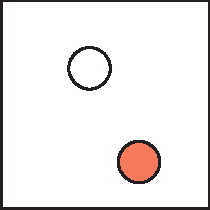
\includegraphics[width=5cm]{figs/samplefigure}
   \caption{Arquitetura do Programa.}
  \label{Fig1}
\end{figure}
 
\subsection{Artefatos}
\label{SebSec:Artefatos}
Os artefatos entregues devem ser documentados no relatório:
\begin{itemize}
\item Arquivos contidos no programa. Lista dos nomes dos arquivos, assim como a extensão dos arquivo
\item Aquivo README, com instruções de uso do software desenvolvido e necessidades técnicas para a execução do programa
\item Arquivos de entrada/saída, caso necessário.
\end{itemize}

